
Science is understanding the world -- $\theta \epsilon \omega \rho \iota \alpha $; art is affecting the world -- $ \pi \rho \alpha \xi \iota \sigma $.
Outreach for scientists is a matter not just of connecting with colleagues in the academy, as C.P. Snow~\cite{SnowTwoCultures} said, bridging the Two Cultures.
It is reaching back to our innate humanity and the world from which it came, the universe trying to understand itself. 
No single exhibit reaches this goal, though we do our best with rubber sheets, lasers, and interactive light and sound sculptures. 
Diligence nonetheless can spark curiosity.
LIGO has made concerted efforts to reach further into the universe with ever more sensitive technology, and in leadup to the World Science Festival exhibit on LIGO in 2010 in Manhattan, we tenaciously developed more sophisticated exhibits to connect with a broader audience. 

    \section{Prototypes: travelling kiosks and the Ann Arbor Hands-On Museum} 
    \label{prototypes}

        Prototypes: Ann Arbor Hands-On Museum and travelling kiosk.

    \textbf{Bill of materials}

\textit{Interferometer parts}

Equipment necessary to construct one interferometer for our Ann Arbor Hands-On
Museum outreach design, including company names, part numbers, quantities, and
prices, after the work done in 2008 by Ramon Armen. Assembly follows from the
work available through

\url{http://gallatin.physics.lsa.umich.edu/~keithr/outreach/}, 

in particular the parts list 

\url{http://gallatin.physics.lsa.umich.edu/~keithr/outreach/LIGOExhibitParts_2.doc},

and the schematic 

\url{http://gallatin.physics.lsa.umich.edu/~keithr/outreach/ifo_schematic.jpg}.

CVI Melles-Griot: 1 505 296 9541; press 2 at menu \\
Description     Part Number     Quantity   Approximate Unit Price\\
HeNe laser      05 LLR 811-249  1          \$320 \\
Laser stand     07 LHE 001      1          \$40 \\

Edmund Optics: 1 800 363 1992; press 1 (?) for sales \\
Description     Part Number     Quantity   Approximate Unit Price\\
-50 lens        NT32-996        1          \$27 \\
-25 lens        NT32-992        1          \$27 \\
Lens holder     NT54-980        2          \$33.00\\

OptoSigma: 1 949 851 5881 
Description     Part Number     Quantity   Approximate Unit Price\\
Beam splitter   038-0590        1          \$250\\
Retroreflector  055-2340        2          \$289.00\\
"" holder       113-0045        2          \$69.00\\

ThorLabs: 1 973 579 7227; press 1 (?) for sales\\
Description     Part Number     Quantity   Approximate Unit Price\\
BS holder       LMR2            1          \$23.50\\
Rotary mount    RP01            1          \$91.00 \\
1.0" holder     PH1-ST          1          \$7.03\\
1.5" holder     PH1.5-ST        4          \$7.22\\
0.75" post      TR075           1          \$4.74 \\
1.0" post       TR1             4          \$4.74 \\
Screw base 1    BA1S            6          \$5.13\\
Screw base 2    BA1             1          \$5.56 \\

Moreover, the following screws will prove necessary:

Type            Length          Quantity\\
1/4"-20 capped  5/4"            8\\
1/4"-20 capped  3/4"            7\\
1/4"-20 set     3/8"            5\\
\#8-32   set     1/2"            1\\

        \begin{figure}
        \begin{center}
        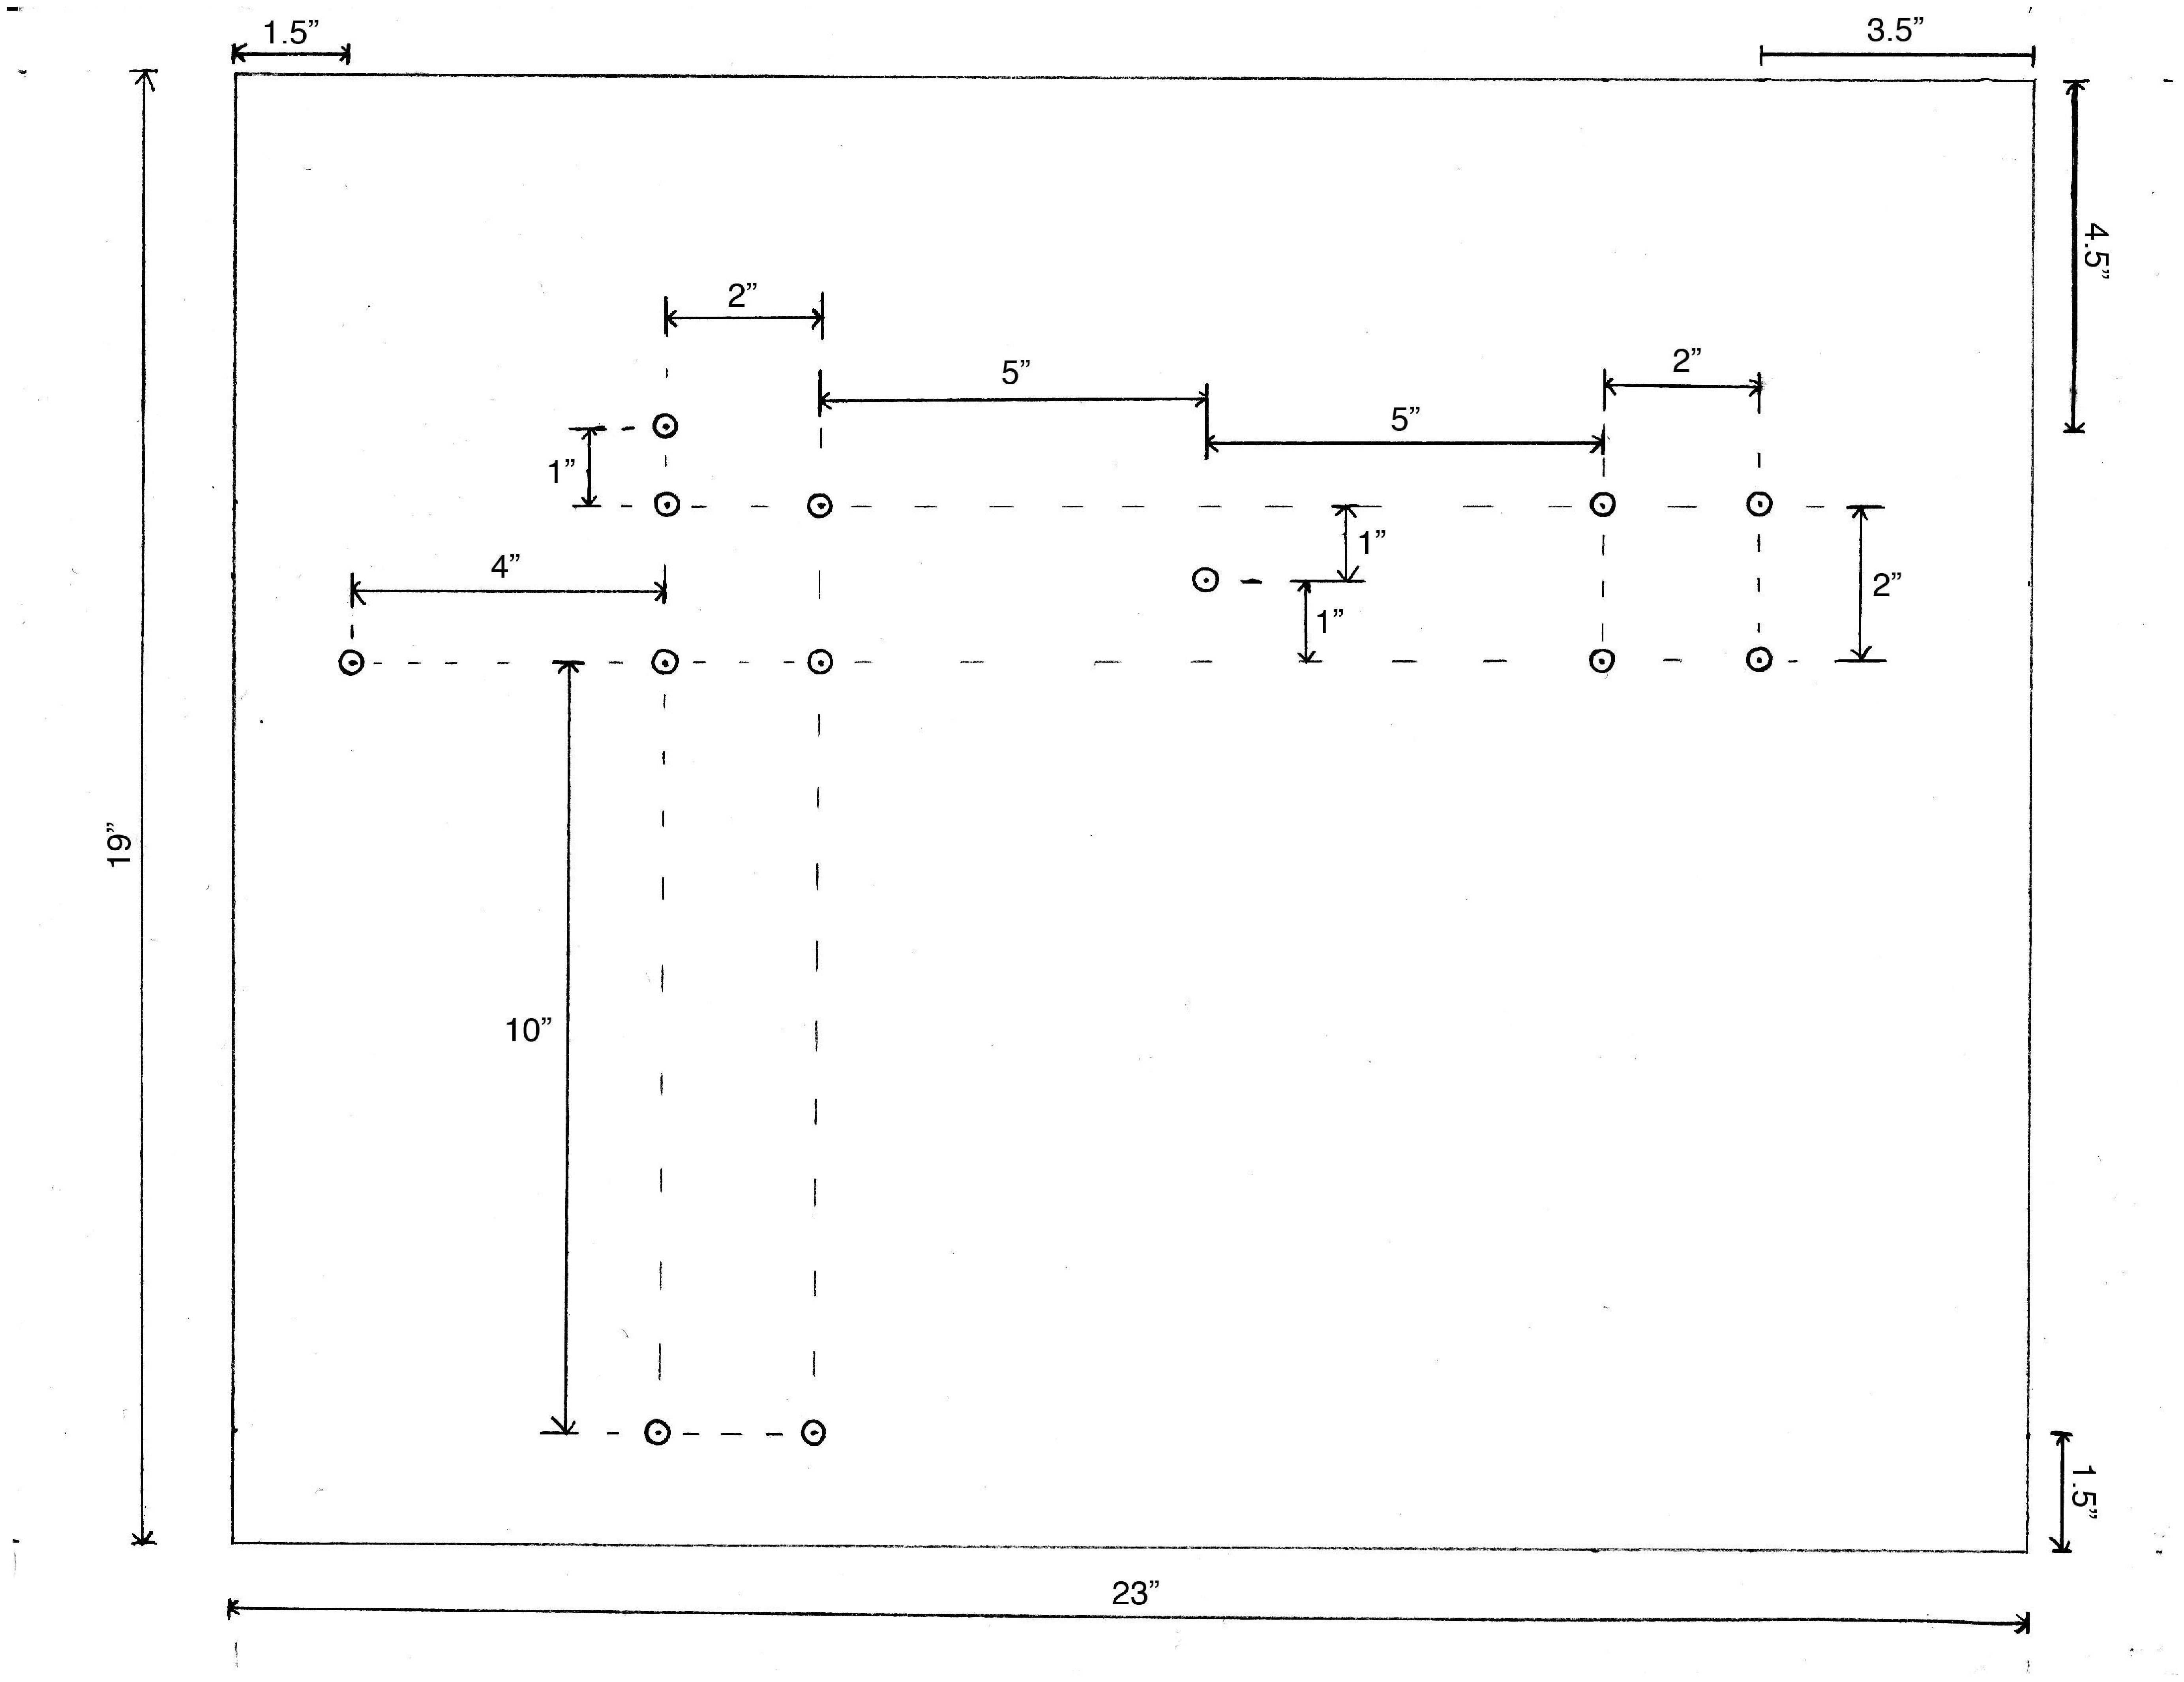
\includegraphics[height=120mm, width=160mm]{ifo_schematic.eps}
        \caption{Kiosk interferometer schematic}
        \label{kiosk_ifo_schematic}
        \end{center}
        \end{figure}

Figure~\ref{kiosk_ifo_schematic} shows the base structural dimensions of this kiosk interferometer.


    \section{World Science Festival interferometer manufacture}
    \label{manufacture}

        World Science Festival interferometer in isolation.

    


        \subsection{Laser, optics and display}
        \label{laser_display}

            Laser and optics (and display).

	\begin{figure}
	\begin{center}
	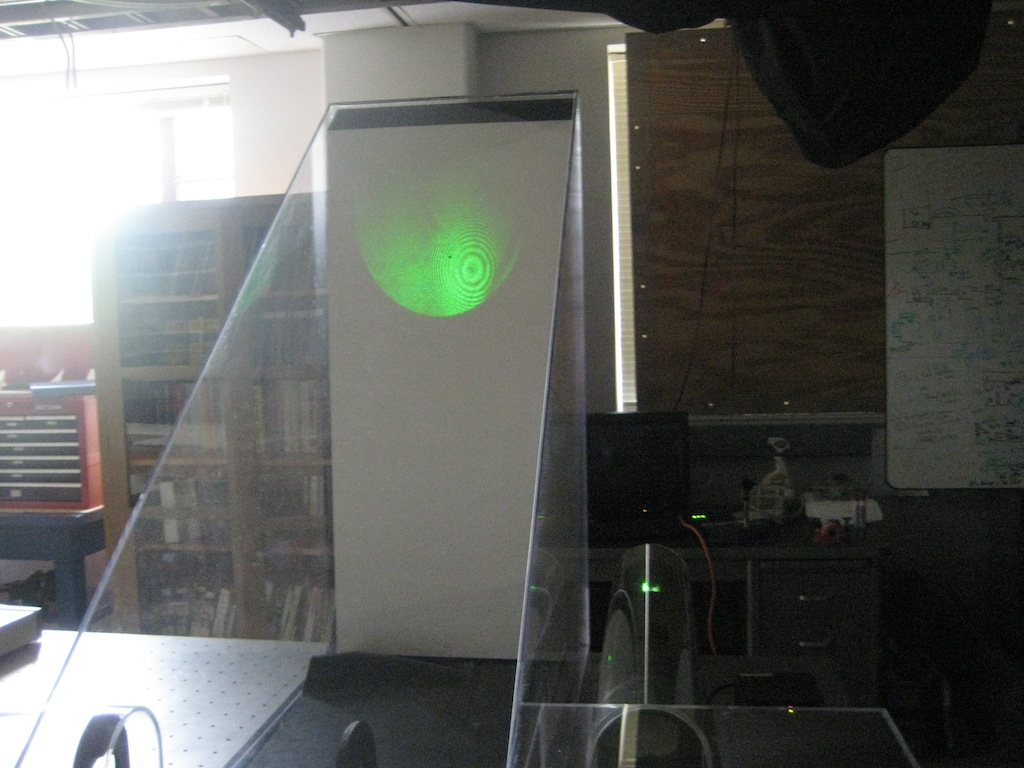
\includegraphics[height=120mm, width=160mm]{WSF_AA_fringes.eps}
	\caption{Interferometer fringes during construction in Ann Arbor}
	\label{WSF_AA_fringes}
	\end{center}
	\end{figure}


        \subsection{Aluminum baseboard}
        \label{baseplate}

            Aluminum base plate.

Table~\ref{aluminum_baseboard_hole_locations} references the positions of holes in the aluminum baseboard that must be tapped. These holes permit the attachment of plexiglass blocks with perpendicular screw tappings that in turn allow the attachment of the plexiglass enclosure described in Section~\ref{enclosure}.

\begin{table}[t]
\begin{tabular}{ r r }
10 & 80\\
04 & 18\\
04 & 12\\
04 & 10\\
08 & 10\\
12 & 12\\
12 & 10\\
10 & 12\\
10 & 10\\
10 & 08\\
10 & 06\\
12 & 04\\
10 & 02\\
44 & 10\\
46 & 10
\end{tabular}
\caption{Hole locations (in inches from origin) for the WSF interferometer aluminum baseboard, plotted on Figure~\ref{al_top_plate}.}
\label{aluminum_baseboard_hole_locations}
\end{table}

        \subsection{Plexiglass enclosure}
        \label{enclosure}

            Plexiglass, many lessons learned.

        \begin{figure}
        \begin{center}
        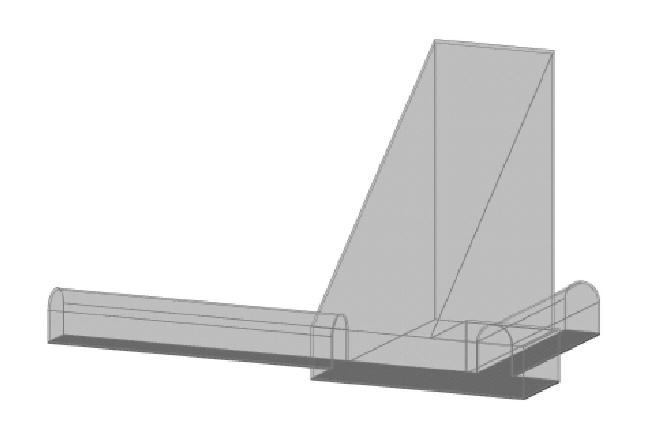
\includegraphics[height=60mm, width=100mm]{view-corner.eps}
        \caption{Corner view of plexiglass and aluminum interferometer enclosure.}
        \label{plex-view-corner}
        \end{center}
        \end{figure}

        \begin{figure}
        \begin{center}
        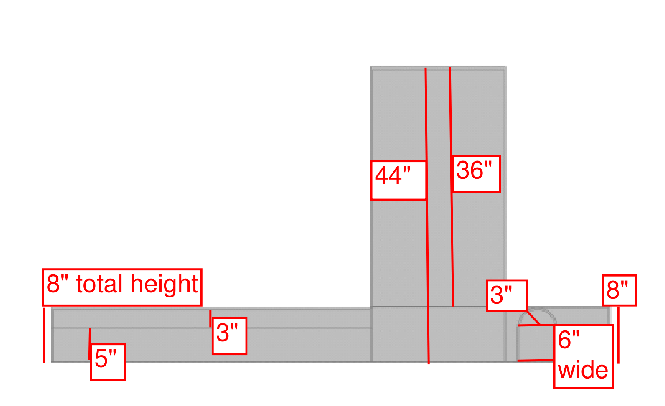
\includegraphics[height=60mm, width=100mm]{view-front.eps}
        \caption{Front view of interferometer aluminum and plexiglass enclosure, with dimensions.}
        \label{plex-view-front}
        \end{center}
        \end{figure}



        \begin{figure}
        \begin{center}
        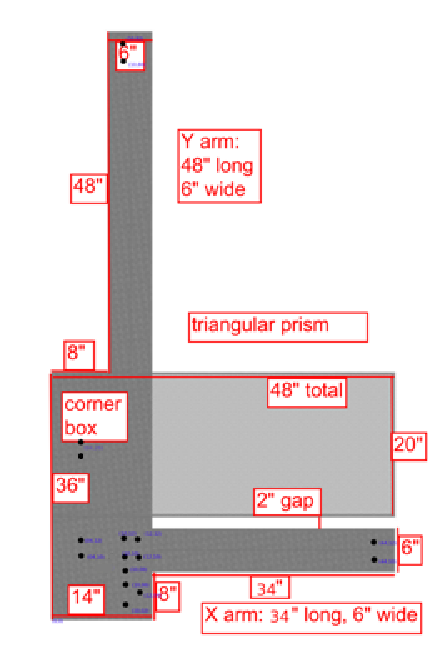
\includegraphics[height=80mm, width=50mm]{view-top-plate-3.eps}
        \caption{Dimensions and hole locations of the aluminum plate (dark gray) relative to plexiglass (light gray), with precise hole locations given by Table~\ref{aluminum_baseboard_hole_locations}.}
        \label{al_top_plate}
        \end{center}
        \end{figure}


	\begin{figure}
	\begin{center}
	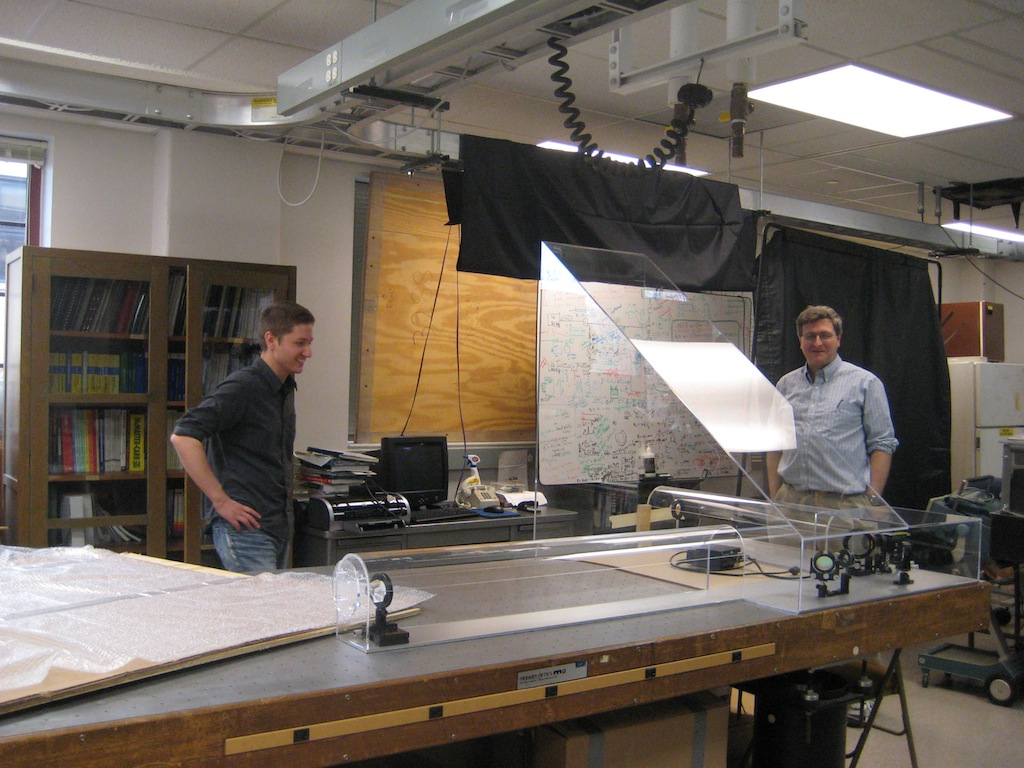
\includegraphics[height=120mm, width=160mm]{WSF_under_construction.eps}
	\caption{Inteferometer assembly in Ann Arbor, Michigan.}
	\label{WSF_in_AA}
	\end{center}
	\end{figure}

Should calculate lower bound on $h(t)$ sensitivity based on Saulson, compare to Robert Forward's interferometer.


    \section{Exhibitions: New York City, Portsmouth, Fort Wayne}
    \label{exhibitions}

        World Science Festival interferometer installed.

	\begin{figure}
	\begin{center}
	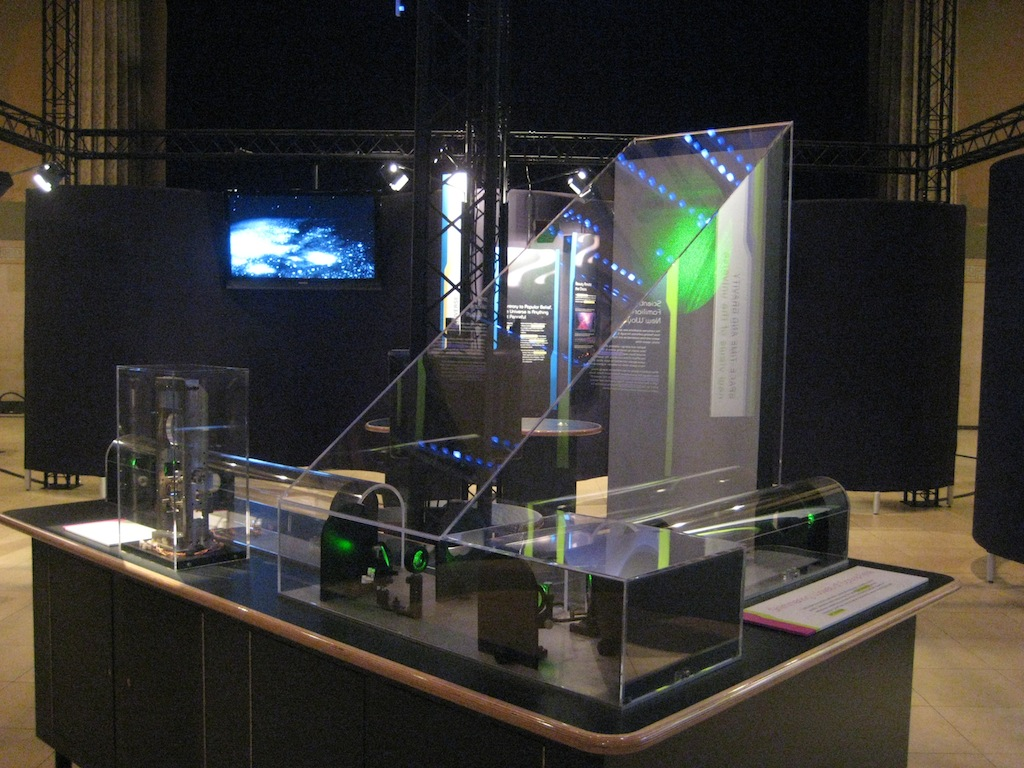
\includegraphics[height=120mm, width=160mm]{WSF_in_NY.eps}
	\caption{World Science Festival interferometer installed in the New York City exhibition hall, June 2010.}
	\label{WSF_IFO_photo}
	\end{center}
	\end{figure}


        \subsection{Exhibit overview}
        \label{exhibit_overview}

            NYC exhibit overview: design, walls, kiosks, displays, interactivities.

        \subsection{World Science Festival 2010}
        \label{WSF2010}

            Success in WSF 2010.

	\begin{figure}
	\begin{center}
	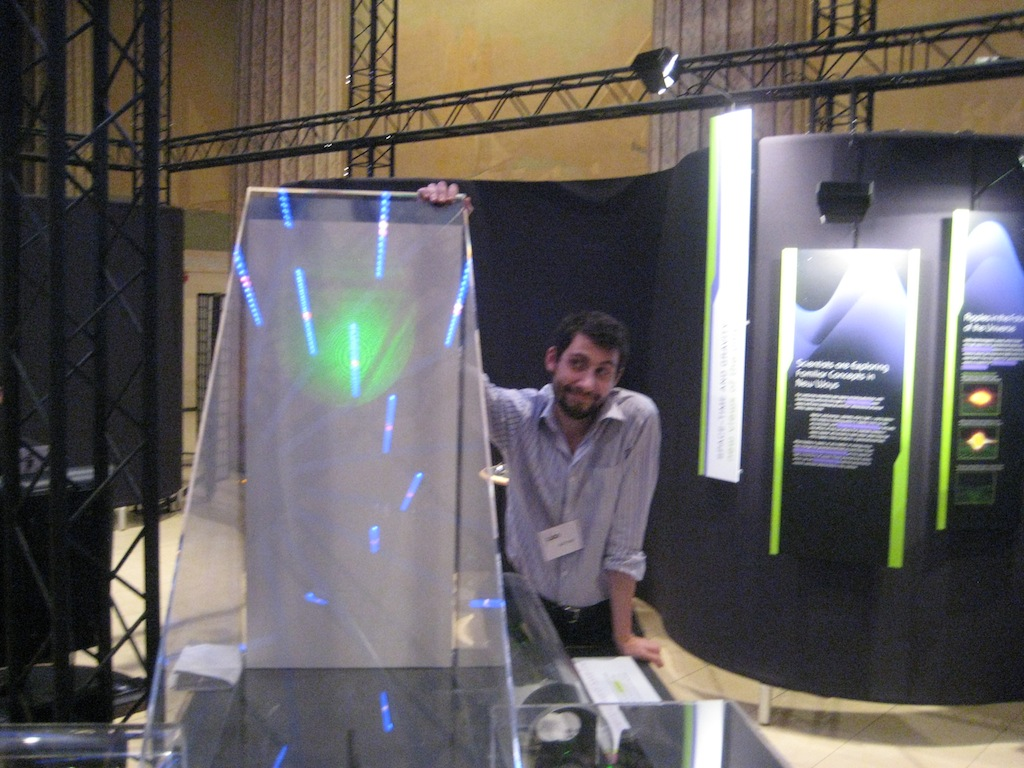
\includegraphics[height=120mm, width=160mm]{WSF_me_NY.eps}
	\caption{Helping to host the exhibit at the World Science Festival.}
	\label{WSF_IFO_me}
	\end{center}
	\end{figure}


        \subsection{Portsmouth and Fort Wayne}
        \label{secondary_installations}

            Secondary installations and future outreach potential.

    \section{Future LIGO outreach}
    \label{future_outreach}

        Epilogue: as of June 2014, the exhibit is safely on display in the Livingston Science and Education center.

        Future LIGO outreach? How to explain a new astronomy.


        --------------------------------------

	%The following is an example of using the commands \textit{ref}
	%and \textit{label}. With these commands theorems, chapters,
	%sections and figurres can be labeld with names in the tex file
	%and then refered to by these names in later tex files. In
	%chapter~\ref{intro} we saw section~\ref{sample_section} or
	%theorem~\ref{sample_theorem}.

	%Lastly, here is how to include a figure. First generate an
	%encapsulated postscript file in xfig, adobe illustrator or
	%some other program. The specific commands are found in
	%\textit{chap2.tex}.

        %\begin{figure}[htb]
        %\centerline{ \epsfig{figure=sample.eps, 
        %height =  1.5 in}}
        %\caption{Sample Figure}
        %\label{sample_figure}
        %\end{figure}

